\chapter{Classification Approaches}

A classifier is a tool that tries to categorize unseen patterns in suitable classes.\newline
An accurate (or a "good") train-set is crucial to build a model that provides the best accuracy to Anomaly Detection.\newline
The classifier uses the train-set to build the model that will be used to classify users (and programs) behaviour and to take decision about whether the observed actions are legitimate or not. Empirical studies will help in choosing the most accurate model (in terms of false-positives and false-negatives ratio)\newline\newline

Here there are the most used approached towards classification in Anomaly Detection:

\begin{itemize}
	\item \emph{Decision Trees} are certainly one of the most used and accurate tools for classification. It builds a model from a train-set that takes decision based on the comparison between the observed features and the nodes of the tree, starting from the root until reaching a decision (leaf) node
	\vspace{0.3cm}
	\item \emph{Nave Bayes} simply uses a form of Bayesian Network to infer intrusions
	\vspace{0.3cm}
	\item \emph{Support Vector Machine} is a technique in which we try to minimize the risk (but we sacrifice some accuracy) in order to optimize speed and scalability
	\vspace{0.3cm}
	\item \emph{Neural Network} is a "connectionist" approach that tries to simulate the human's brain with artificial (digital) neurons. The pros of this approach is, no doubt, its accuracy when the network is trained for a long period, consisting in multiple generations of NN. The cons is that if an error is made in the first generations, it will be propagated to the next ones
	\vspace{0.3cm}
	\item \emph{K-Nearest Neighbours} is the simplest approach (but surprisingly one of the most accurate in the field of Intrusion Detection!) among all these Machine Learning techniques. The idea is to classify "patterns" instead of features
\end{itemize}

Collecting some results from empirical studies, here it is a comparison table from all these classification approaches combined with the feature selections technique. As can be seen, the \emph{Decision Tree} classification technique is the one with the \emph{overall} best accuracy.\newline
On the other hand we got the best accuracy combining K-NN with Information Gain

\begin{figure}[h!]
	\centering
	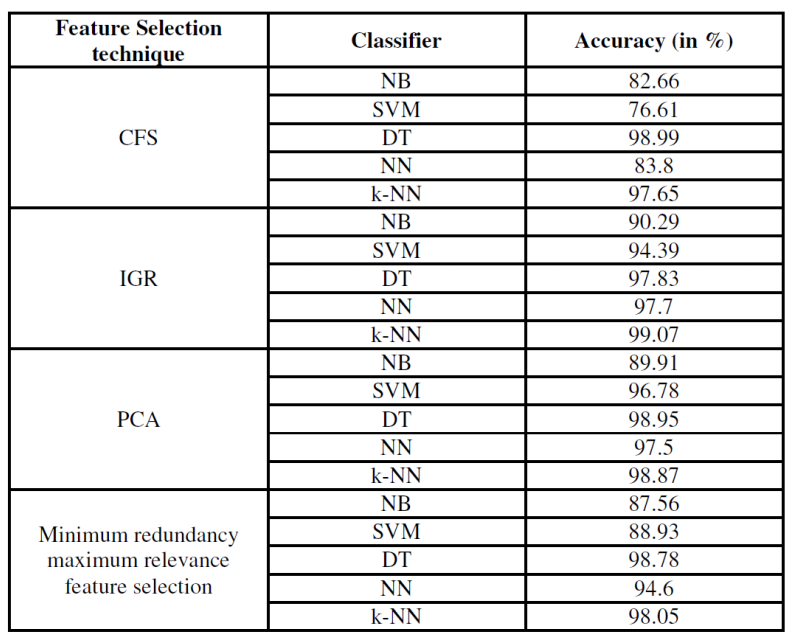
\includegraphics[width=\textwidth]{img/Comparison.png}
\end{figure}